% !TEX root = root.tex
\chapter{\label{chap:methods}Experimental Methods}
\chaptermark{Methods}

\section{Experimental Challenges in Interfacial Particle Tracking}

\subsection{Colloidal Aggregation at the Interface}

When microrheological probes aggregate, the colloidal aggregate does not retain the simple geometry of an individual colloid and therefore is of no further use in the experiment. It is straightforward to visually identify aggregated probes and disregard them in the analysis. But each aggregation event depletes the population of usable probes and limits the experiment's duration.

This problem is especially acute in interfacial experiments because, at the air--water interface, microrheological probes have an enhanced tendency to aggregate. The van der Waals interaction between partially-immersed colloids is more complex than their interaction in bulk solution, which itself is complicated\cite{Crocker1994}; but, on a basic level, the strength of the attraction is intermediate with respect to strengths of the interactions in the two pure phases. Particles at the air--water interface interact more strongly than submerged particles due to the dry portion. As a point of reference, for polystrene spheres, there is seven-fold difference in the strength of van der Waals attraction between fully submerged and unsubmerged colloids\cite{Williams1991}. Additionally, the stabilizing electrostatic repulsion between charge--stabilized colloids diminishes as it de-wets, which further magnifies the net attraction\cite{Williams1991,Lyne1989}. The attraction may also be increased by a depletion interaction driven by the adsorbed molecules under study (in this case, proteins or bacterial byproducts). Finally, while the capillary attraction of ``floating'' particles is the most obvious driver of aggregation at the interface, it is weak for the systems in this study, which are characterized by a low Bond number $\Delta\rho g^2/\gamma$. However, it may be enhanced if the contact line along the particle is rough.

In this work, the charge--stabilized colloids used (see methods sections of respective chapters for details) did indeed aggregate throughout the experiment. However, the evolving mechanical properties of the interface under study often inhibited colloidal mobility as the interface stiffened and effectively arrested aggregation before the population of unaggregated probes could be completely depleted. Some control could be exerted over the aggregation rate by varying the salt concentration of the bulk solution and by adjusting the concentration of dispersed colloids. At lower concentrations, the colloids are of course less likely to encounter each other, and aggregation proceeds more slowly.

\subsection{Distinguishing Interfacial Particles}

When colloidal probes are spread onto the interface, many can be pinned there, but some invariably enter the bulk solution. As they undergo random diffusion in the bulk, they may approach the interface, where they can easily be mistaken for particles that are at the interface. Thus, in interfacial particle-tracking experiments, it is important to critically examine individual particles, considering whether particles exhibiting an anomolous appearance or anomolous motion may not be attached to the interface. This has been an important, if mundane, challenge to address in this work. It has recently been emphasized in the literature by others\cite{Samaniuk2014}, and part of the motivation for developing flexible particle-tracking software (Chapter \ref{chap:trackpy}) that makes this detailed work easier.

\subsection{Minimizing and Correcting for Convective Drift}

When possible, the chamber containing the sample should be well sealed to minimize sample evaporation and convective flow during the experiment\cite{Savin2005}. In interfacial microrheology experiments, convective flow is an especially large effect, as the interface can couple strongly to surrounding air currents. In the data analysis stage, the effect of such currents can be corrected for\cite{Crocker2007}, but it is best to minimize it in the experiment as much as possible. The experiment should be performed on a vibration-isolated table. Like convective drift, vibrations can be ``removed'' in the analysis stage, but not perfectly.

\subsection{Choosing an Appropriate Particle Concentration}

Obviously, the more particles that are in the fields of view and are tracked, the better the resulting statistics; however, there are additional considerations. As mentioned above, the particle concentration affects the rate of particle aggregation, but there are other considerations as well. The concentration must be appropriate for tracking individual particles. The average particle spacing must be larger than the average particle displacement from frame to frame, or else the paths of multiple particles will intermingle, making it difficult to accurately reconstruct individual trajectories\cite{Crocker1996}. (In some circumstances, it is possible to overcome this limitation, as described in Section \ref{sec:prediction}.)

Additionally, the presence of the colloidal probes themselves can alter the self-diffusivity of the probes through hydrodynamic interactions\cite{Peng2008a}, which are longer-range in 2D than in 3D ($\log(r)$ vs. $1/r$). Experimental measurements of the diffusivity of PMMA particles showed that diffusivity $D$ decreased with area fraction $n$ like

\begin{equation}
D = \alpha D_0(1 - \beta n)
\end{equation}

\noindent where $D_0$ is the diffusivity for a single particle. For particles 1 \textmu m in diameter, $\alpha$ is compatible with 1 (reported as $0.97 \pm 7\%$) and $\beta = 1.4 \pm 10\%$\cite{Peng2008a}. Thus, if spherical colloidal probes are dispersed with an area fraction of 3\%, the resultant error in diffusivity is less than 5\%, which is small compared to other experimental uncertainties in this work.

\section{Experimental Apparatus}

All interfacial microrheology experiments described in this thesis were performed in a cylindrical ``cell'' designed to create flat interface air--water or oil--water interface using only a small volume of sample. This cell (Figure \ref{fig:cell-and-quarter}) is a short cylinder: 4 mm high with a 1-cm inner diameter. A seam runs along the waist of the inner surface, 2 mm above the bottom surface, composed of aluminum below and Teflon above. When the cylinder is filled precisely up to this seam with an aqueous solution, the solution is pinned flat by the aluminum-Teflon boundary. There is no meniscus. A glass coverslip serves as a bottom to the cell, through which the interface can be imaged using an inverted microscope. (The interface can also be imaged from above using a standard microscope, as in Chapter \ref{chap:bacteria}.) This coverslip is held in place by a thin coat of vacuum grease, applied to the bottom surface of the cylinder. Alternatively, a grease-free seal can be made using a custom-molded PDMS sheath that seals the outer surface of the cell to the glass below.

   \begin{figure}
    \centering
    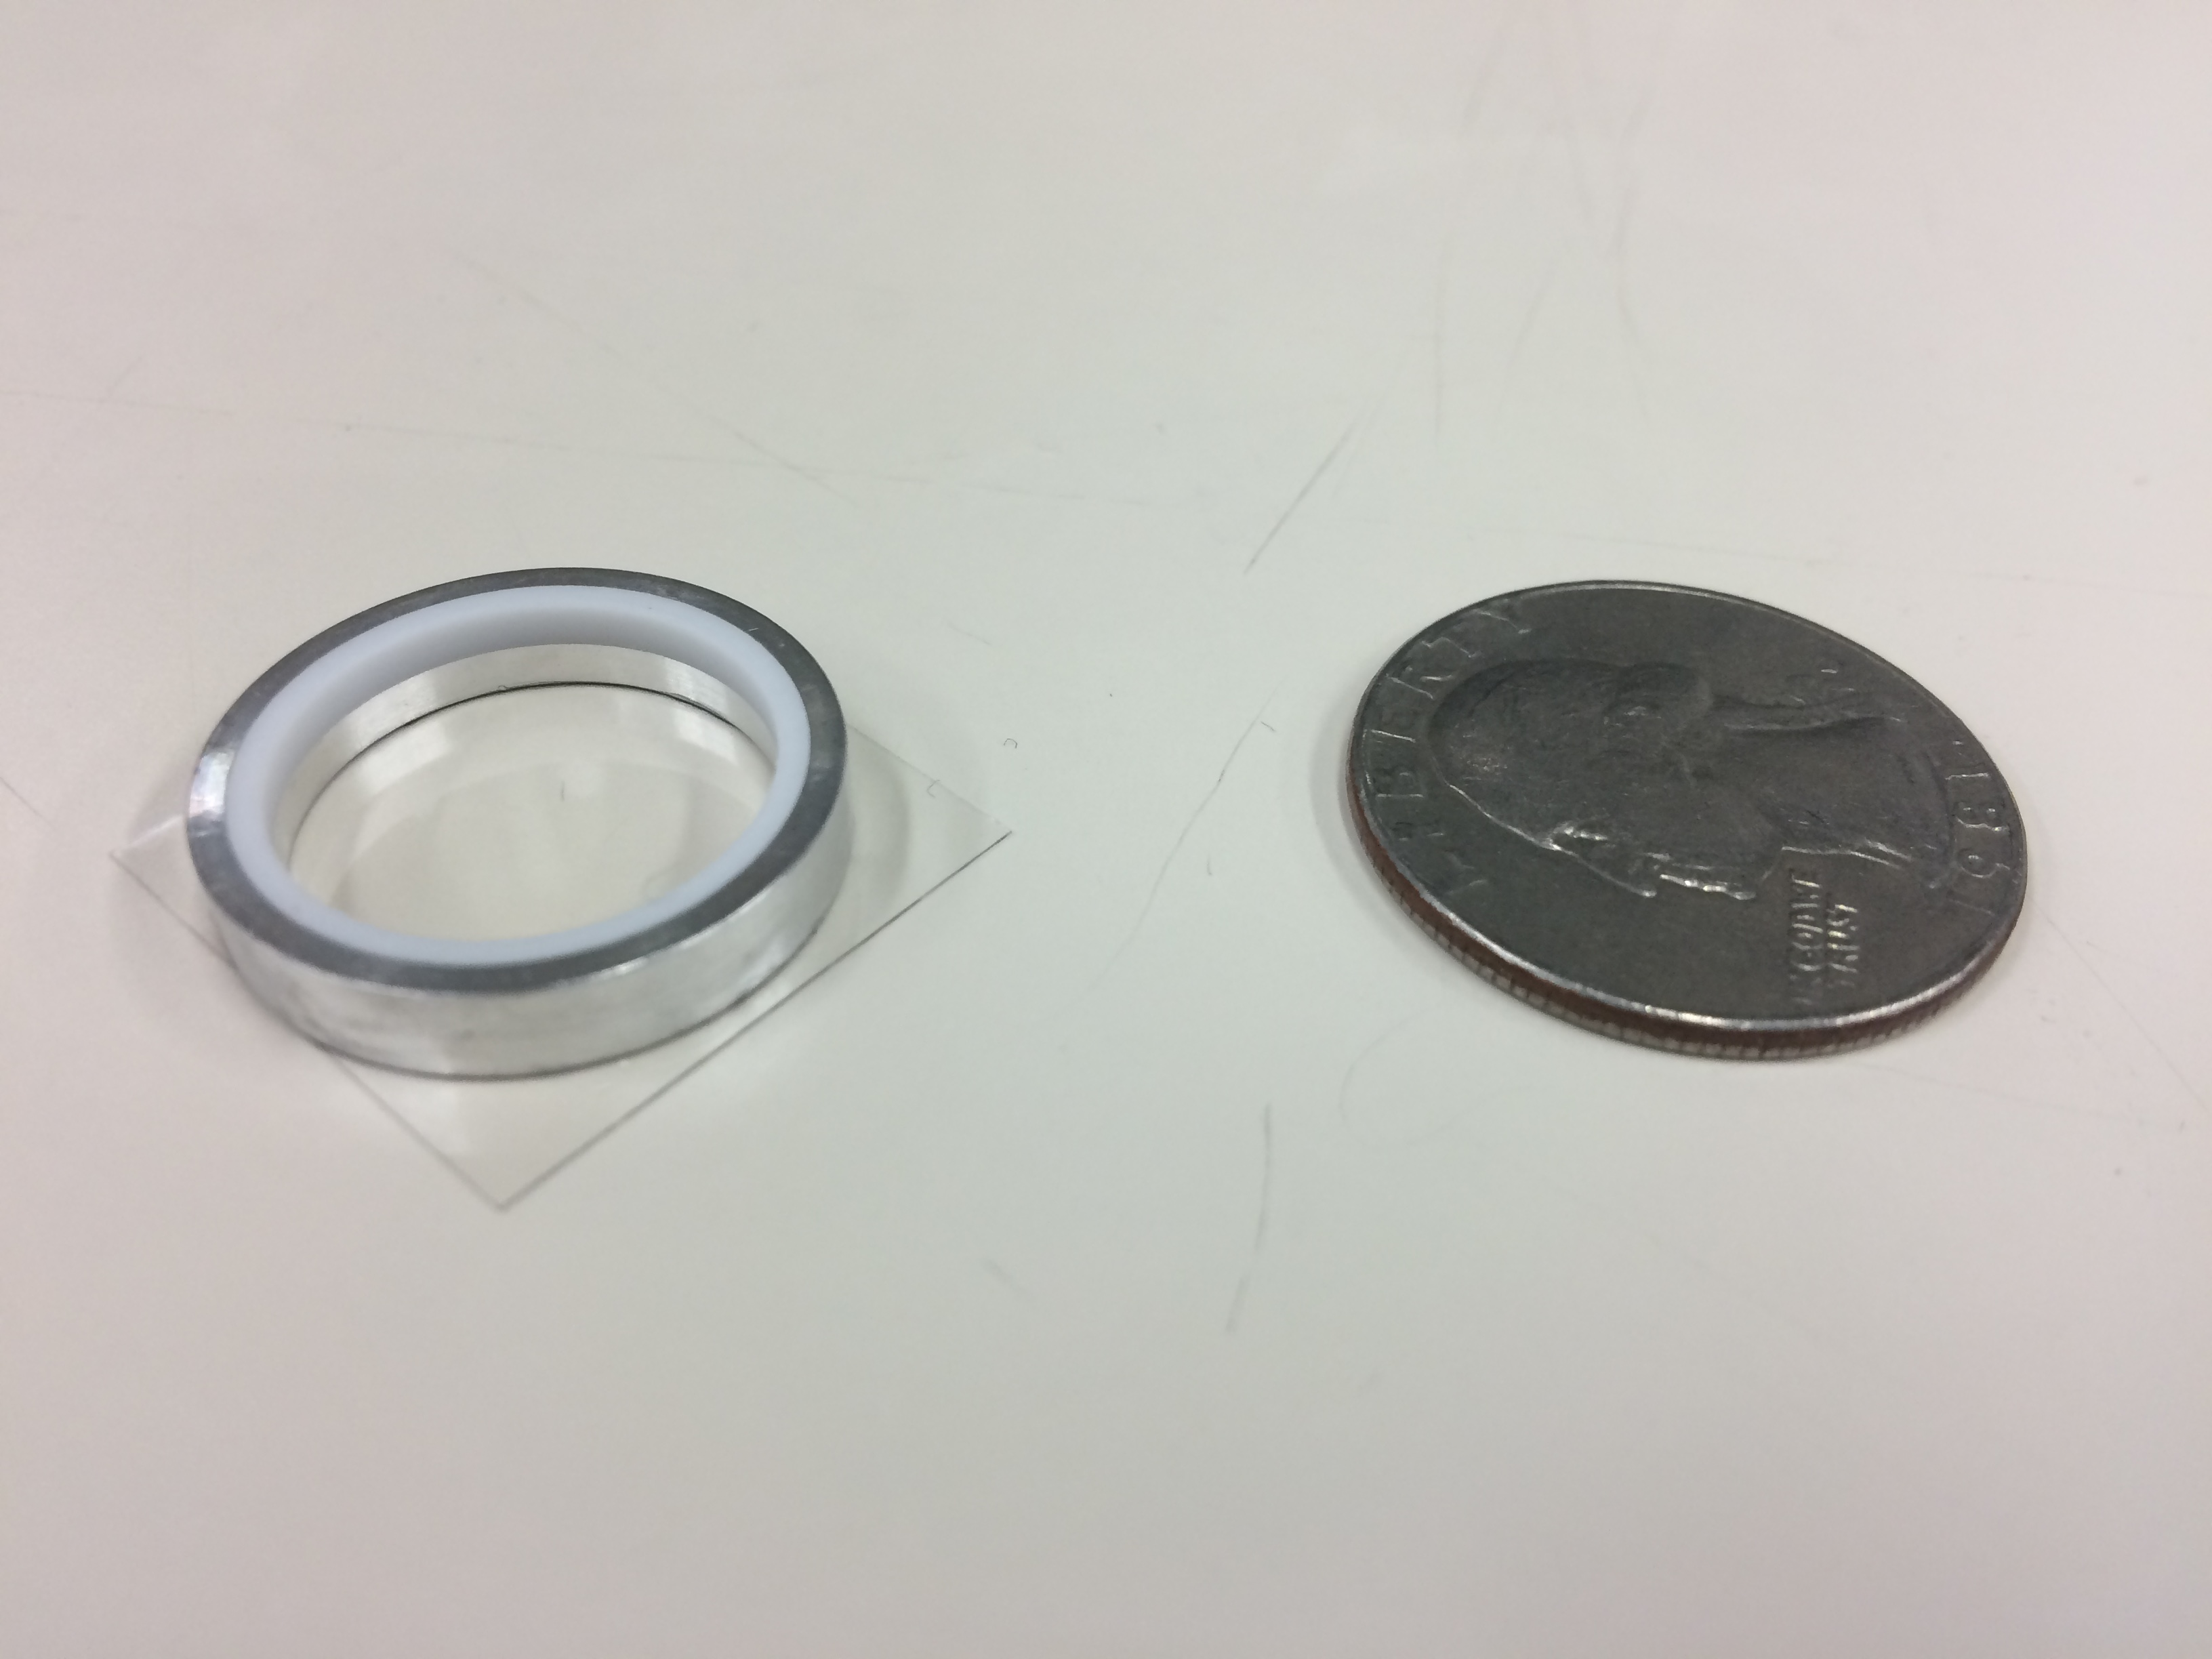
\includegraphics[width=\columnwidth]{methods/cell-and-quarter}
    \caption{\label{fig:cell-and-quarter}The experiments in this thesis were performed in the cylindrical Teflon and aluminum cylinder at left. The Teflon--aluminum seam on the inner surface pins the air--water or oil--water interface flat. A glass coverslip forms the bottom, attached and sealed using a thin coat of vacuum grease. A quarter is shown for scale.}
    \end{figure}

Consumer-grade cameras are sufficient for some bright-field particle-tracking applications, delivering the same basic capabilities as scientific cameras---frame rate, resolution---at a fraction of the cost. (In fluorescent particle-tracking experiments, where sensitivity is paramount, special cooing and readout electronics are more important.) In a previous study and in preliminary experiments leading to this work, our lab used a ``point-and-shoot'' consumer camera (Nikon COOLPIX 4300). The sensor was physically small, which led to greater noise, and the video data was compressed in a way that can distort motion. For the study described in Chapter \ref{chap:lysozyme}, to increase the signal-to-noise ratio and improve the fidelity of the video data, this was replaced by a digital SLR-style consumer camera (Nikon D3100) with a larger sensor and the capability of exporting uncompressed video. Data from these consumer-grade cameras was supplemented with data from a scientific camera capable of high frame rates (Photron Fastcam 512) and, for the experiments described in Chapter \ref{chap:snase}, a high-resolution scientific camera (IOIndustries Flare 4M). The studies described in Chapters \ref{chap:bacteria} and \ref{chap:photoactivation} were performed using hardware described in detail in their respective sections on experimental methods.

\section{Ferromagnetic Nickel Nanowires}

\subsection{Overview of Fabrication and Characteristics}

Ferromagnetic nickel nanowires were fabricated for use in active microrheology experiments. The wires can be made 5--35 \textmu m long (10\% length polydispersity\cite{Hultgren2004,Hultgren2005}) with a diameter of $350 \pm 40$ nm\cite{Hultgren2004,Hultgren2005}. Because their diameters are comparable to the characteristic size of a magnetic domain in bulk nickel and their aspect ratio is high, the wires possess a single magnetic domain over their entire volume, aligned with the long axis. Their remnant magnetization is 70\% of the saturation of bulk nickel\cite{Sun1999} with a magnetic moment per unit length of $3.0 \times 10^{-14}\pm0.6\% \,\text{A}\cdot\text{m}^2$/\textmu m. Thus, they couple strongly to externally applied magnetic fields, and they act as strong, robust probes of soft--matter systems.

The wires were fabricated by electrochemical deposition inside the pores of a nanoporous template: a ceramic filter, obtained commercially and repurposed for this technique. The detailed protocol has been described both in published literature\cite{Chien2002} and a thesis\cite{TanaseThesis}.

The dominant source of the uncertainty in the figure for $\mu/L$ cited above is the uncertainty in the wire diameter. The length can be estimated in visually in brightfield experiments, but the diameter cannot. The variation in magnetization under experimentally applied fields is relatively small\cite{Hultgren2004,Hultgren2005}. For more detailed characterization of the wire's magnetic properties, see the referenced literature.

\subsection{Hydrophobic Functionalization}

The nickel nanowires are functionalized to create a more hydrophobic surface. When they are dispersed across the air--water interface, plain nickel wires would sink, but hydrophobially functionalized wires are pinned at the interface and can remain stably at the interface for many hours. The nanowires are functionalized in a mixture of 0.01 ml \emph{n}-octadecyltrimethoxysilane (OTMS), 0.01 ml ammonium hydroxide, and 10 ml ethanol. The wires are soaked this mixture for 12 hours. Then, after at least three rises in pure ethanol, the wires are dispersed in isopropyl alcohol (being a cleaner solvent than ethanol) for storage and use. The air--water contact angle is $79 \pm 1^\circ$ at an OTMS-functionalized surface, as measured using a goniometer (Rame-Hart, P/N 100)\cite{Lee2010} to photograph a water droplet on a plate on functionalized nickel. Typically, protocols like this one use centrifugation to recover the colloids between rinses. Because the wires are ferromagnetic, they can conveniently be separated from the solution by merely holding a magnet against the wall of the container for a few seconds and then pouring off the liquid. Alternative schemes for hydrophobic functionalization are available in the literature\cite{Sugimura2002,Fond2007}.

\section{Tracking Nanowire Orientation}

The raw data of our active microrheology experiment is a series of video microscopy images of a nanowire. The orientation of the wire must be extracted from the images. Although the orientation is plain to any human observer, an automated solution is required due to the sheer volume of data ($10^5$ images) and the necessity of precise and consistent judgements of an angular trajectory through time. The analysis is deceptively difficult to automate. We have developed a family of approaches, each with certain advantages. The important metrics are precision, robustness, and performance (speed).

A standard algorithm for identifying line segments in an image is the Hough Transform. Unfortunately, this is completely ineffective on our data. Although the wires are rods with a high aspect ratio, diffraction effects cause them to appear more like fuzzy ellipses that straight lines.

The simplest effective technique is to fit an ellipse to the wire's silhouette. A threshold defines regions inside and outside the wire, and a least-squares best fit obtains the ellipse that most accurately encloses that region. The orientation of the ellipses long axis is the orientation of the wire. This is typically accurate within 1$^\circ$ and it is robust---it virtually always captures orientation within 10$^\circ$---but it is not precise enough to track the wire's rotation smoothly.

A more precise technique is to fit a Gaussian to each individual row or column of pixels in the image, where each Gaussian's center identifies the position of the wire along that line. The linear regression of the Gaussian centers gives the centerline of the wire. This technique is precise but quite slow. Worse, it is brittle, prone to completely missing the wire orientation in noisy or otherwise non-ideal conditions.

The most effective technique is to find the ``inertial axes'' of the image (where brightness = mass). For an image with intensities $\{I_i\}$ at pixels located at ${(x_i, y_i)}$, we compute its covariance matrix $u$

\begin{equation}
\left( \begin{array}{c}
\overline{x} \\
\overline{y} \end{array} \right)
= \left( \begin{array}{c}
\sum_{i} I_i x_i / \sum_i I_i \\
\sum_{i} I_i y_i / \sum_i I_i \end{array} \right)
\end{equation}

\begin{equation}
u = \left( \begin{array}{cc}
\sum_{i} I_i x_i^2 / \sum_i I_i - \overline{x}^2 & \sum_{i} I_i x_i y_i / \sum_i I_i - \overline{x}\,\overline{y} \\
\sum_{i} I_i x_i y_i / \sum_i I_i - \overline{x}\,\overline{y} & \sum_{i} I_i y_i^2 / \sum_i I_i - \overline{y}^2\end{array} \right)
\end{equation}

\noindent from which we can obtain the orientation of the wire,

\begin{equation}
\theta = \frac{1}{2}\tan^{-1}\left(\frac{2u_{11}}{u_{20} - u_{02}}\right).
\end{equation}

\noindent The technique is much faster than fitting Gaussians, and its precision is comparable: both are precise to 0.1$^\circ$. We have also found it to be more robust, though not quite as robust as the ellipse-fitting method.

All of the methods above require standard image preparation techniques. The region of interest is isolated from the surrounding image (the wire is largest connected region of bright pixels). The image is gently blurred with a Gaussian kernel of width about 1 pixels to suppress the jagged effect of camera noise, and distant background pixels are clipped to black, but immediate neighborhood of the wire is retained.